% Overizcht feest:
% Datum 24-07-2017
% Aantal gasten 45
% Waarvan kinderen 5
% Betreft: Diversen

% Begintijd: 13:00
% 

\documentclass{scrartcl}
\usepackage[dutch]{babel}
\usepackage{fancyhdr}
\usepackage{wallpaper}
\usepackage[official]{eurosym}
\usepackage{background}
\usepackage{url}
\usepackage{enumitem}
\setlist{nosep, after=\vspace{\baselineskip}}

% weird character support (ie sate).
\usepackage[utf8]{inputenc}
\usepackage[T1]{fontenc}
\usepackage{lmodern} % load a font with all the characters


\setcounter{secnumdepth}{0}% % Turns off numbering for sections
\makeatletter
\usepackage{etoolbox}% http://ctan.org/pkg/etoolbox
\patchcmd{\@sect}% <cmd>
  {\else \protect}% <search>
  {\protect\numberline{}\else\protect}% <replace>
  {}{}% <success><failure>
\makeatother 

\graphicspath{{img/}}

\backgroundsetup{
  scale=1.2,
  color=black,
  opacity=1,
  angle=0,
  position=current page.south,
  vshift=110pt,
  hshift=50pt,
  contents={%
  \begin{minipage}{.8\textwidth}
	\center
	\large Restaurant De Huiskamer \\
	\tiny Kerkdijk 2 - 7964KB Ansen - tel 0522-471280 - KvK 04005343 -  info@dehuiskamer.com \\
	IBAN NL07 SNSB 095.65.49.721 - BTW nr: 8094.43867B01 \\
	\url{www.dehuiskamer.com} - \url{www.de2dekamer.nl} - \url{www.facebook.com/RestaurantDeHuiskamer}
  \end{minipage}\hspace{-.05\textwidth}%
  \begin{minipage}{.18\textwidth}
  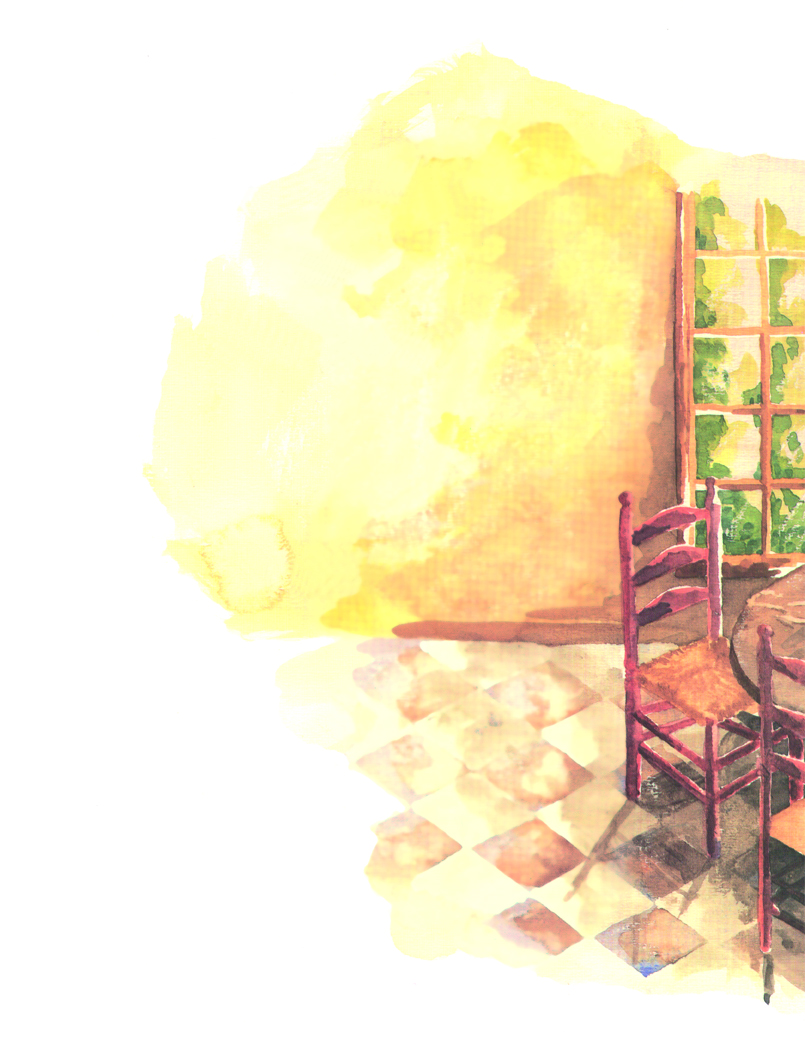
\includegraphics[width=\linewidth,height=110pt,keepaspectratio]{logo2kleur}
  \end{minipage}%
  }
}

\pagestyle{fancy}
\cfoot{}
\renewcommand\headrulewidth{0pt}
\chead{\large Restaurant De Huiskamer \\
\small Ansen $\quad$ tel $0522-471280$}
\begin{document}
\ThisURCornerWallPaper{0.25}{img/logo.jpg}

\title{Restaurant De Huiskamer}
\date{Ansen, \today}
\maketitle
\thispagestyle{empty}

\begin{flushright}
	Tietsje v.d. Beek \\
	Wilhelminastraat 4 \\
	9073 HB Marrum
\end{flushright}
\section{Betreft: offerte}
\begin{tabular}{l r}
  E-mail & tietsje@hotmail.com  \\
  Tel & 06-28092108  \\
\end{tabular}

\subsubsection*{Geachte mevrouw
 Tietsje v.d. Beek,}

Naar aanleiding van ons gesprek ontvangt u hierbij een vrijblijvend offerte voorstel
voor een Diversen
 op 24-07-2017 \\

Uitgaande van 45 gasten incusief 5 kinderen kan dit er als volgt uit zien: \\\\
\begin{tabular}{ll} 
13.00 uur & 1e gang high tea \\
14.00 uur &  Borrelen \\
15.00 uur & Hightea De Huiskamer in buffet vorm \\
16.30 uur & Soepbuffet\\
17.00 uur & Einde \\

 \end{tabular} 


\newpage

\subsection*{Kosten specificatie}
Uigaande van 45 gasten inclusief 5 kinderen.

\begin{tabular}{l l l r l r} 
135 & Consumpties/Borrelen & \euro{} & 2.30 & \euro{} & 310.50 \\
40 & Hightea De Huiskamer & \euro{} & 22.90 & \euro{} & 916.00 \\
5 & Kinderen & \euro{} & 17.20 & \euro{} & 86.00 \\
\hline
& Totaal incl. btw & & & \euro{} & 1312.50 \\
\end{tabular} 


\subsection*{Bijzonderheden}

-

\begin{itemize} 
	\item Consumptie prijs is een gemiddelde van alle dranken (behalve buitelands gesistileerd).
 
	\item Bij deze offerte gaan we uit van 25 volwassen gasten.
 
	\item Kinderen tot 4 jaar eten gratis mee. Tussen de 4 en 12 krijgen korting.
 
	\item Voor meer informatie kunt u ook terecht op www.de2dekamer.nl
 
\end{itemize} 


We hopen uw wensen op de juiste wijze te hebben vertaald, in afwachting op uw reactie, \\

Met gastvije groet, \\\\

Pedro Klooster

\newpage

\section{Activiteit details}

